\section{Experimental results}

For our experiments we use the \emph{Caltech-15} dataset, a digital image dataset containing about 2537 images  split between 15 distinct object categories (faces, watches, elephants, motorbikes, etc.)\footnote{\emph{Caltech-15} has been created at the \emph{California Institute of Technology}}. Image descriptors are precomputed over the whole dataset and stored on separate files.. All tests were performed on a Mac OSX Notebook with an Intel Core i5, 8GB (running at 2.4 GHz).

Tests have been made on varying of these parameters: train set size, vocabulary size and SIFT descriptor type (\emph{dense, sparse, multi-scale}). At least a comparison between \emph{hard} and \emph{soft assignment} is presented. Test set size is always set to 30 (30 images from each category).

In Table \ref{tab:trainsetsize} the classification accuracies on varying training set size (the number shown represent how many images taken from each category) are shown. As we can see in Table \ref{tab:trainsetsize} the larger the training set size the better accuracy is obtained due the greater number of examples used to create the model.

\begin{table}[h]
\begin{center}
\begin{tabular}{|l|c|c|c|}
\hline
 & 10 & 30 & 50\\
\hline\hline
NN $L_2$ & 38,44 & 53,33 & 52,06\\
NN $\chi^2$ & 59,67 & 67,33 & 67,74\\
SVM Linear & 57,56 & 72,44 & 76,58\\
SVM IK & 72,44 & 79,33 & 83,53\\
SVM $\chi^2$ & 72,44 & 79,56 & 83,27\\
SVM RBF & 57,56 & 71,78 & 72,31 \\
\hline
\end{tabular}
\end{center}
\label{tab:trainsetsize}
\caption{Classification accuracies on varying training set size}
\end{table}

In Figure \ref{fig:vocabulary} it is shown the classification accuracies variation on growing vocabulary size. All tests have been made fixing training set size to 30 and using \emph{dense SIFT}. Generally the greater the number of codewords used the greater the accuracy obtained.

\begin{figure}[h]
\begin{center}
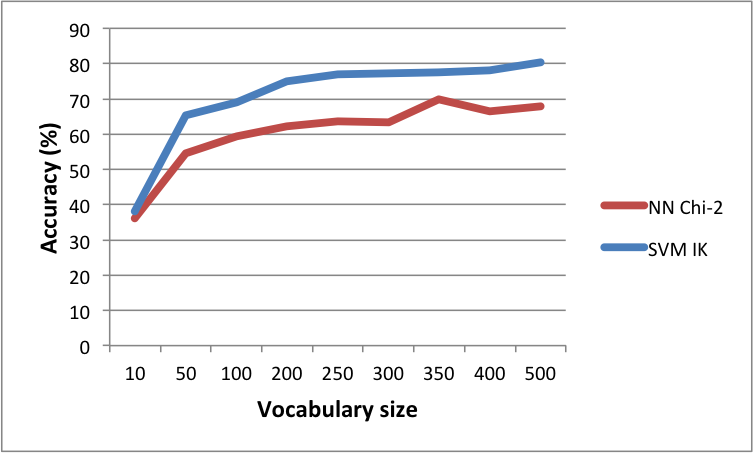
\includegraphics[width=0.45\textwidth]{images/vocabulary.png}
\end{center}
  \caption{Classification accuracies on growing vocabulary size}
\label{fig:vocabulary}
\end{figure}


